\documentclass[a4paper,14pt,twoside,onecolumn,openany,final]{memoir}

% Page Layout
\setlrmarginsandblock{1.5in}{1in}{*}
\setulmarginsandblock{1in}{*}{1}
\checkandfixthelayout[nearest]

\usepackage{graphicx, xcolor, titling, hyperref}
\hypersetup{
    colorlinks=true,
    linkcolor=blue,
    filecolor=magenta,
    urlcolor=cyan,
  }
\usepackage{amsmath, amssymb, amsthm, mathtools}

\usepackage{minted}

\graphicspath{{images/}}

% line spacing
\OnehalfSpacing
%\linenumberfrequency{1}
%\bvnumbersoutside
%\bvtopandtail
%\setverbatimfont{\normalfont\ttfamily\small}

% page style
\pagestyle{plain}
\chapterstyle{demo2}

\author{Sandesh Thakuri}
\title{Finite Difference Method in MATLAB}
\date{Jan, 2024}
%---------------------------------------------------------------------------------------------------------------
\begin{document}

\frontmatter
\vspace{2cm}

\begin{center}
  {\bfseries { \LARGE
      \vspace{2cm}


      {\color{blue}{\thetitle}}}

    \vspace{1cm}

    {\large{\color{red!90}{For PDEs: Heat Equation, Advection-Diffiusion Equation,...}}



      \vspace{1.5cm}

      {\color{blue}{Tutor}}: \hspace{6mm} Dr. Jeevan Kafle \\
      {\color{blue}{Compiled by}}: \hspace{5mm} Mr. \theauthor\\


      \vspace{2cm}

      
\includegraphics[scale=0.9]{logo.jpg}

      \vspace{2cm}

      Centeral Department of Mathematics\\
      TU, \; Nepal\\
      \thedate\\
    }}
\end{center}
\thispagestyle{empty}
\clearpage
\begin{center}
  {\LARGE{\bfseries Acknowledgement}}
\end{center}

\vspace{1.5cm}
{\large
  First, I would like to thank Mr. {\bfseries Hari Babu Khatri} for helping me with the figures and Ms. {\bfseries Roshina Shrestha} for providing me the old codes.\\ \\

  Then I would like to thank Mr. {\bfseries Bikram Bhandari} and Mr. {\bfseries Nabin Niraula} for helping me out with the errors. Finally, I would like to thank my whole class for the positive feedback. Also, I am thankful for our teacher Dr. Jeevan Kafle.\\

  Thank You.\\ \\

}
\begin{flushright}
  \theauthor \\
  \thedate
\end{flushright}


\clearpage


\tableofcontents
%-------------------------------------------------------------------------------------------------------------------------------
\mainmatter

\part{Finite Difference}
\chapter{Finite Difference}
In this method we discretize a space into a finite number of points and use these points to find an
approximate solution of a PDE.

 \section{Schemes for Discretization}
Let $u=u(x,t)$ be a function in two variables. \\ \\
Let the interval of the variable $x$ is discretized into $m$ number of points; $x_1,x_2,...,x_m$ and
of the variable $t$ into $n$ number of points; $t_1, t_2,...,t_n$. \\

 \subsection{Forward Difference of \(1^{st}\) order}
 \[\frac{{\partial u}(x_i,t_j)}{\partial x} = \frac{u(x_i+h,t_j)-u(x_i,t_j)}{h} =
 \frac{V_{i+1}^j - V_i^j}{h}\]
 Likewise,\\
 \[\frac{\partial u}{\partial t} = \frac{V_i^{j+1}-V_i^j}{k}\] \\

 \subsection{Backward Difference of \(1^{st}\) order}
 \[\frac{{\partial u}(x_i,t_j)}{\partial x} = \frac{u(x_i,t_j)-u(x_i-h,t_j)}{h} =
 \frac{V_i^j - V_{i-1}^j}{h}\]
 Likewise,\\
 \[\frac{\partial u}{\partial t} = \frac{V_i^j-V_i^{j-1}}{k}\]\\

 \subsection{Central Difference of \(1^{st}\) order}
 It is the average of forward difference and backward difference.\\
 \[\frac{{\partial u}(x_i,t_j)}{\partial x} = \frac{V_{i+1}^j - V_i^j + V_i^j - V_{i-1}^j}{2h} =
 \frac{V_{i+1}^j - V_{i-1}^j}{2h}\] \\

 \subsection{Central Difference of \(2^{nd}\) order}
 \[\frac{\partial^2 u}{\partial x^2} = \frac{V_{i+1}^j-2V_i^j+V_{i-1}^j}{h^2}\]

 \[\frac{\partial^2 u}{\partial t^2} = \frac{V_i^{j+1}-2V_i^j+V_i^{j-1}}{k^2}\]

 \vspace{2cm}
 \subsection{Code Conventions:}
 \begin{table}[h!]

     \begin{tabular}{||c c c c c||}
     \hline
     Variables & Axis & Loop var. & difference & Grid section \\ [0.5ex]
     \hline\hline
     x & X & i & h & m \\
     t/y & Y & j & k & n \\[1ex]
     \hline
     \end{tabular}
    \end{table}


 \chapter{Heat Equation}
 Forward time Central space Scheme \textbf{(FTCS)} for the heat equation: \(u_t= \alpha u_{xx}\).\\
 We have,

\begin{align*}
 \frac{\partial u}{\partial t} &= \alpha \frac{\partial^2 u}{\partial x^2} \\
 \frac{V_i^{j+1}-V_i^j}{k} &= \frac{V_{i+1}^j-2V_i^j+V_{i-1}^j}{h^2} \\
 V_i^{j+1}-V_i^j &= \frac{\alpha k}{h^2} (V_{i+1}^j-2V_i^j+V_{i-1}^j) \\
 V_i^{j+1} &= V_i^j+c (V_{i+1}^j-2V_i^j+V_{i-1}^j)
 \end{align*}

 where \( c=\frac{\alpha k}{h^2} \). This the required scheme.
 \vspace{1cm}

\subsection{Question}
\begin{align*}
    u_t&= \alpha u_{xx}           &   0<x<1, \;\; t>0, \;\; \alpha=0.05\\
    BCS:\;\; u(0,t) &= u(1,t)=0   &   t>0\\
    IC:\;\; u(x,0)  &= sin{\pi}x  &   0<x<1
\end{align*}
\clearpage

\section{Matlab Code}
  \begin{minted}[frame=lines,framerule=3pt, framesep=10pt, fontsize=\small, linenos]{matlab}
%initialization
L=1;      m=10;   h=L/m;    x=0:h:L;
T=1;      n=10;   k=T/n;    t=0:k:T;

a=0.05;       c=a*k/(h*h);
v=zeros(m+1, n+1);

%checking
if (c<0|c>0.5)
  disp('The FTCS is unstable.');
else

%boundary equations
  v(1,:)=0;     v(m+1,:)=0;
  v(:,1)=sin(pi*x);

%scheme
  for j=1:n
    for i=2:m
      v(i,j+1)=v(i,j)+c*(v(i+1,j)-2*v(i,j)+v(i-1,j));
    end
  end
end

%graph
[p,q]=meshgrid(x,t);

surf(p,q,v);
xlabel('x');  ylabel('y');  zlabel('z');
title('Numerical solution of heat equation.');
\end{minted}

\chapter{Advection Diffusion Equation}
Forward Time Backward Space Central Space Scheme (FTBSCS) for the following advection diffiusion equation:\\
\[\frac{\partial C}{\partial t} + v\frac{\partial C}{\partial x} = D\frac{\partial^2 C}{\partial x^2}\]
where,\\
C is concentration of disolved sustances \\
v is velocity of the fluid \\
D is diffussion coefficient. \\ \\

We have,
\begin{align*}
  \frac{V_i^{j+1}-V_1^J}{k} + v\frac{V_i^j - V_{i-1}^j}{h} &= D\frac{V_{i+1}^j-2V_i^j+V_{i-1}^j}{h^2}\\
  V_i^{j+1}-V_1^j &= \frac{Dk}{h^2}(V_{i+1}^j-2V_i^j+V_{i-1}^j)-\frac{vk}{h}(V_i^j - V_{i-1}^j)\\
  V_i^{j+1} &= F(V_{i+1}^j-2V_i^j+V_{i-1}^j)-G(V_i^j - V_{i-1}^j)
\end{align*}

where,\\
\(F=\frac{Dk}{h^2}\) \hspace{5mm} \(G= \frac{vk}{h}\)

\subsection{Question}
\begin{align*}
  C_t + vC_x &= D C_{xx} \\
  0 \leq t &\leq 4000*24,          &       D=10^{-6}*3600\\
  0 \leq x &\leq 100,          &       v=10^{-7}*3600\\
  IC: \;\; C(x,0) &= 100
\end{align*}

\section{Matlab Code}

\begin{minted}[frame=lines,framerule=3pt, framesep=10pt, fontsize=\small, linenos]{matlab}
%Initialization
L=100;    m=20;   h=L/m;    x=0:h:L;
T=4000*24;  n=20;   k=T/n;  t=0:k:T;

D=(1E-6)*3600;      F=(D*k)/(h*h);
V=(1E-7)*3600;      G=(V*k)/h;

v=zeros(m+1,n+1);

%Initial conditon
v(:,1)=100;

%Scheme
for j=1:n
  for i=2:m
    v(i,j+1)=v(i,j)+F*(v(i+1,j)-2*v(i,j)+v(i-1,j))-G*(v(i,j)-v(i-1,j));
  end
end

%Graph
[p,q]=meshgrid(x,t);
surf(p,q,v);
xlabel('x';    ylabel('y');    zlabel('z');
title('Numerical solution of Advection-Diffusion equation.');
\end{minted}
\begin{figure}
\centering
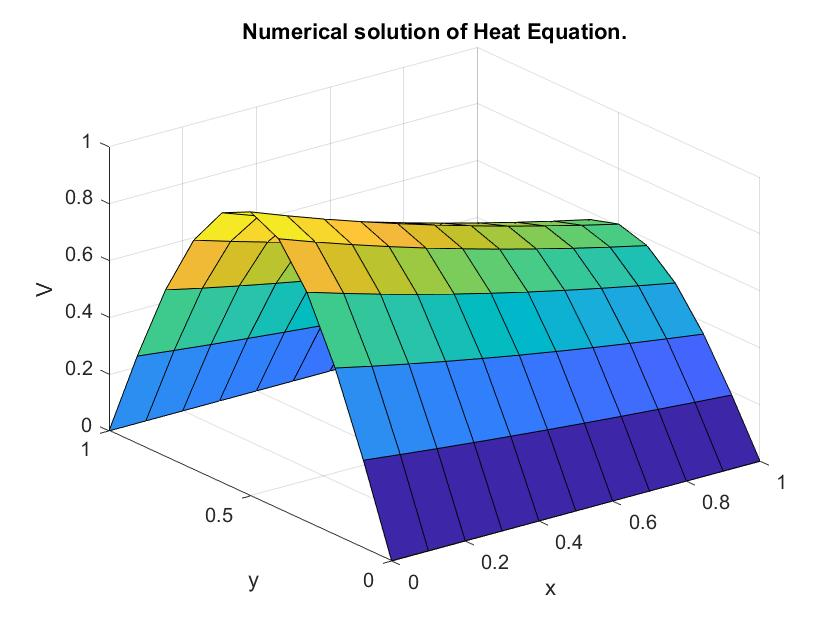
\includegraphics[scale=0.4]{heat.jpg}
\caption{Heat Equation}
\end{figure}
\begin{figure}
  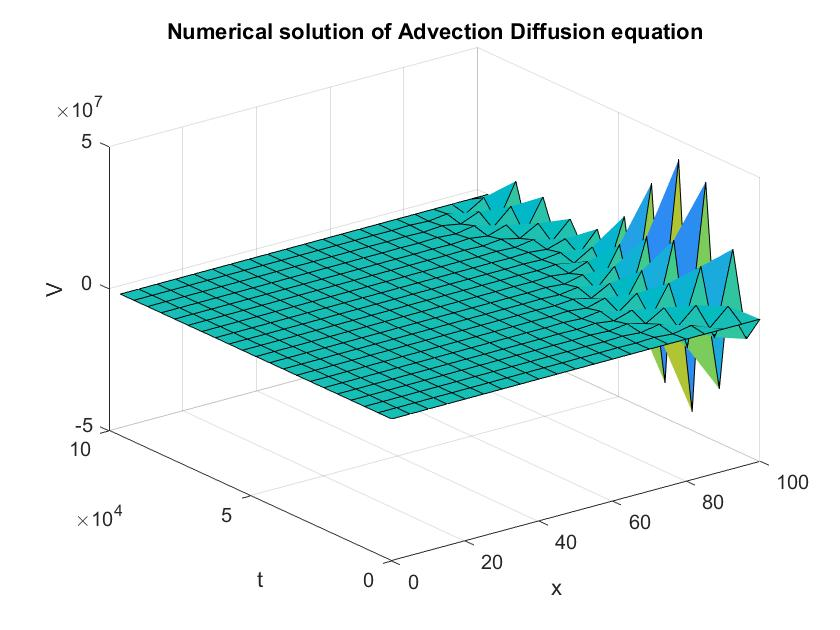
\includegraphics[scale=0.4]{advection.jpg}
  \caption{Advection Diffiusion equation}
\end{figure}
\chapter{Laplace Equation}

The Laplace equation is
\[ u_{xx}+u_{yy}=0 \]

The Central Space Central Space Scheme (\textbf{CSCSS}) for the above equation:

\begin{align*}
  \frac{V_{i+1}^j-2V_i^j+V_{i-1}^j}{h^2} + \frac{V_i^{j+1}-2V_i^j+V_i^{j-1}}{k^2} &= 0\\
  k^2(V_{i+1}^j-2V_i^j+V_{i-1}^j) + h^2(V_i^{j+1}-2V_i^j+V_i^{j-1}) &= 0\\
  k^2(V_{i+1}^j+V_{i-1}^j) + h^2(V_i^{j+1}+V_i^{j-1}) &= 2(h^2+k^2)V_i^j\\
\end{align*}
\begin{equation}
  V_i^j = \frac{k^2(V_{i+1}^j+V_{i-1}^j)+h^2(_i^{j+1}+V_i^{j-1})}{2(h^2+k^2)}
\end{equation}

\subsection{Question}
\begin{align*}
    u_{xx}&=u_{yy}           &   0\leq x \leq 2,\;\; 0 \leq y \leq 2\\
    BCS:\;\; u(0,y)&=0, \;\; u(2,y)=5   &   0\leq y \leq 2\\
             u(x,0)&=0, \;\; u(x,2)=-2  &   0\leq x \leq 2
\end{align*}
\clearpage

\section{Matlab Code}
\begin{minted}[frame=lines,framerule=3pt, framesep=10pt, fontsize=\small, linenos]{matlab}
%Initialization
L=2;      m=5;   h=L/m;    x=0:h:L;
B=2;      n=5;   k=B/n;    t=0:k:B;

c=1/(2*(h^2+k^2));
v=zeros(m+1, n+1);

%Boundary Conditions
v(1,:)=0;     v(m+1,:)=5;
v(:,1)=0;     v(:,n+1)=-2;

%Scheme
for j=2:n
  for i=2:m
    v(i,j)=c*((h^2*(v(i,j+1)+v(i,j-1)))+(k^2*(v(i+1,j)+v(i-1,j))));
  end
end

%Graph
[p,q]=meshgrid(x,t);

surf(p,q,v);
xlabel('x');  ylabel('y');  zlabel('z');
title('Numerical solution of Laplace equation.');
\end{minted}
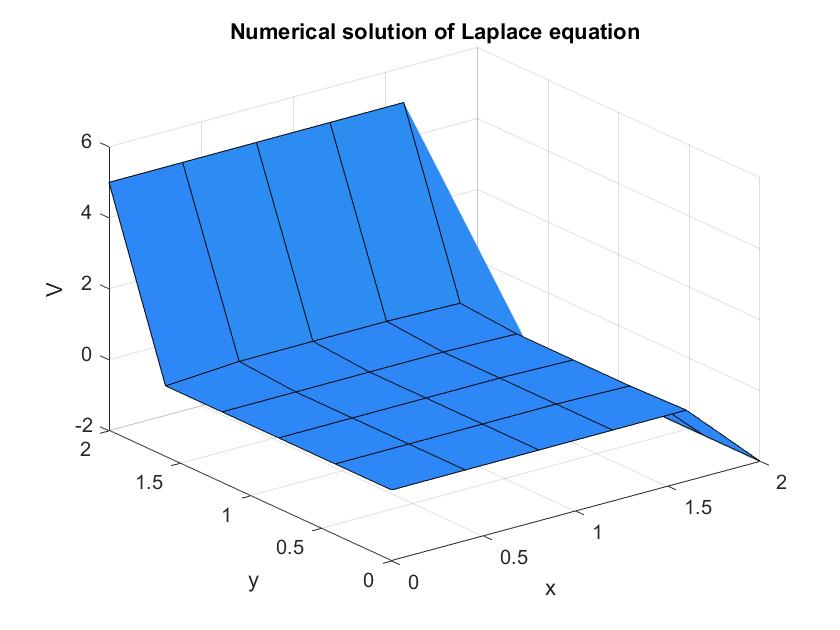
\includegraphics[scale=0.32]{laplace.jpg}

\chapter{Wave Equation}

The wave equation is \hspace{5mm} \(u_{tt}=au_{xx}\) \\ \\

The Central Space Central Space Scheme (\textbf{CTCSS}) for the above equation:

\begin{align*}
  \frac{V_i^{j+1}-2V_i^j+V_i^{j-1}}{k^2} &=  a \frac{V_{i+1}^j-2V_i^j+V_{i-1}^j}{h^2}\\
  V_i^{j+1}-2V_i^j+V_i^{j-1} &= \frac{ak^2}{h^2}(V_{i+1}^j-2V_i^j+V_{i-1}^j)
 \end{align*}
\begin{equation}
  V_i^{j+1} = 2(1-c)V_i^j + c(V_{i+1}^j+V_{i-1}^j)  - V_i^{j-1}
\end{equation}
where, \hspace{5mm} \(c=\frac{ak^2}{h^2}\) \\

\subsection{Question}
\begin{align*}
    u_{tt} &= au_{xx}           &   0 \leq x \leq 1, \;\; t\geq 0\\
    BCs:\;\; u(0,t) &= u(1,t)=0   &   t \geq 0\\
    ICs:\;\; u(x,0)  &= 10sin{\pi}x \hspace{3mm} u_t(x,0)=0  &   0 \leq x \leq 1
\end{align*}

\clearpage

\section{Scheme for Initial Condition}
The initial condition \(u_t(x,0)=0\) also needs a separate scheme as it is in a derivative form.\\

The Central Time Scheme for \(u_t\) is :
\begin{align*}
  u_t =& \frac{V_i^{j+1} - V_i^{j-1}}{2k}\\
  \implies 2ku_t &= V_i^{j+1} - V_i^{j-1}\\
  For j=0 \\
  2ku_t &= V_i^1 - V_i^{-1}
\end{align*}
\begin{equation}
 \implies V_i^{-1} = V_i^1 - 2ku_t
\end{equation}
\\

Also, Putting \(j=0\) in equation (5.1)
\begin{equation}
  V_i^1= 2(1-c)V_i^0 +c(V_{i+1}^0+V_{i-1}^0)  - V_i^{-1}
\end{equation}

From equation (5.2) and (5.3)
\begin{equation}
    V_i^1 = (1-c)V_i^0 +0.5c(V_{i+1}^0+V_{i-1}^0)  +ku_t
  \end{equation}
  \vspace{5mm}
  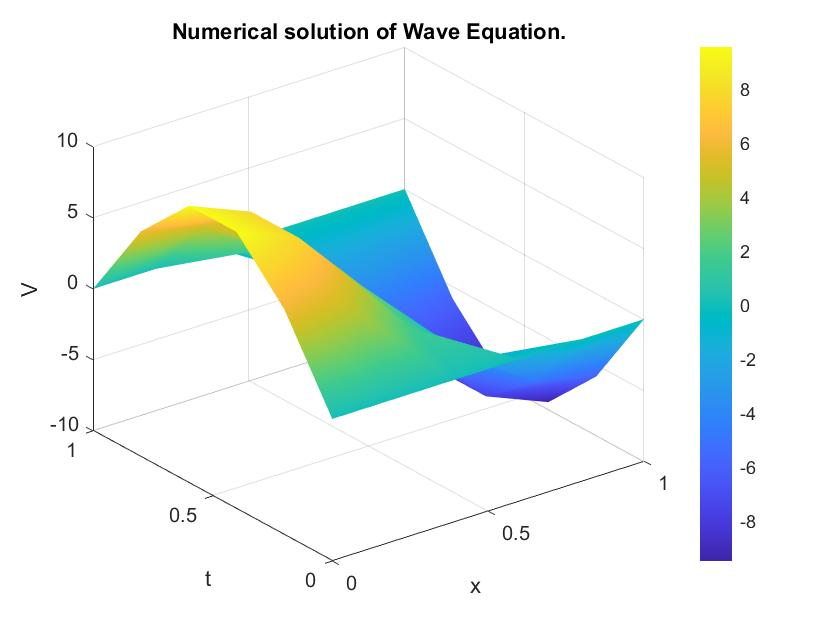
\includegraphics[width=15cm, height=8cm]{wave.jpg}

\clearpage
\section{Matlab Code}
\begin{minted}[frame=lines,framerule=3pt, framesep=10pt, fontsize=\small, linenos]{matlab}
%Initialization
L=1;	m=5;	h=L/m;	x=0:h:L;
T=1;	n=5;	k=T/n;	t=0:k:T;

a=1;			c=a*(k^2/h^2);
V=zeros(m+1,n+1);

%Checking
if (c<=0|c>1)
    disp('The CTCSS is unstable')
else

%Boundary Conditions
    V(1,:)=0;	V(m+1,:)=0;

%Initial Conditions
    V(:,1)=10*sin(pi*x);

    for i=2:m
        V(i,2)=(1-c)*V(i,1)+0.5*c*(V(i+1,1)+V(i-1,1));
    end

%Main Scheme
    for j=2:n
        for i=2:m
            V(i,j+1)=2*(1-c)*V(i,j)+c*(V(i+1,j)+V(i-1,j))-V(i,j-1);
        end
    end

%Graph
    [p,q]=meshgrid(x,t);
    surf(p,q,V,'Edgecolor','none');
    xlabel('x');	ylabel('t');	zlabel('V');
    title('Numerical solution of Wave Equation.');
    shading interp;
end
\end{minted}


\part{Inital Part}

\chapter{Numerical Integartion}
\section{Code for Trapezoidal Rule}
\begin{minted}[frame=lines,framerule=3pt, framesep=10pt, fontsize=\small, linenos]{matlab}

% Initialization
f=@(x) x*sin(x);

a=0;     b=(pi/2);
n=5;     h=(b-a)/n;

S=0.5*(f(a)+f(b));
S1=0;

% Scheme
for i=1:n-1
  xi=a+i*h;
  S1=S1+f(xi);
end

I=h*(S+S1);

fprintf('The integral is %f\n',I)

\end{minted}
\(ans=1.008265\)


\section{Code for Simpson's 1/3 rule}
\begin{minted}[frame=lines,framerule=3pt, framesep=10pt, fontsize=\small, linenos]{matlab}

%Initialization
f=@(x) x*sin(x);

a=0;     b=(pi/2);
n = 12;  h=(b-a)/n;

S=f(a)+f(b);
S1=0;
S2=0;

% Scheme
for i=1:2:n-1
  xi=a+i*h;
  S1=S1+4*f(xi);
end

for i=2:2:n-2
  xi=a+i*h;
  S2=S2+2*f(xi);
end

% Output
I=(h/3)*(S+S1+S2);
fprintf('The integral value is %f.\n',I)

\end{minted}
\(ans=0.999995\)

\clearpage
\section{Code for Simpson's 3/8 rule}
\begin{minted}[frame=lines,framerule=3pt, framesep=10pt, fontsize=\small, linenos]{matlab}

% Initialization
f=@(x) x*sin(x);
a=0;           b=pi/2;     n=12;     h=(b-a)/n;

S1=f(a)+f(b);  S2=0;     S3=0;

% Scheme
for i=1:3:n-2
  x1=a+i*h;
  x2=a+(i+1)*h;
  S2=S2+f(x1)+f(x2);
end

for i=3:3:n-3
  S3=S3+f(a+i*h);
end

% Output
I=(3*h/8)*(S1+3*S2+2*S3);
fprintf('The integral value is %f.\n',I)

\end{minted}

\(ans=0.999989\)


\chapter{Numerical Solution Polynomial equations}
\section{Bisection Method}

\begin{minted}[frame=lines,framerule=3pt, framesep=10pt, fontsize=\small, linenos]{matlab}

%Initialization
f=@(x) x^2-26;
a=5;     b=6;     toll=0.001;

% Scheme
while abs(a-b)>=toll
  c=(a+b)/2;

  if f(a)*f(c)<=0
    b=c;
  else
    a=c;
  end
end

fprintf("The solution by the bisection method is %f.\n",c)
\end{minted}

\(ans=5.098633\)

\clearpage


\section{Newton Raphson's Method}

\begin{minted}[frame=lines,framerule=3pt, framesep=10pt, fontsize=\small, linenos]{matlab}

%Initialization
f=@(x) 3*x*sin(x)-exp(x);
df=@(x) 3*x*cos(x)+3*sin(x)-exp(x);

a0=1;       tollerance=0.0001;   diff=1;

% Scheme
while diff>=tollerance
  a1=a0-f(a0)/df(a0);

  diff=abs(a1-a0);
  a0=a1;
end

fprintf("The solution by Newton Raphson's method is %f.\n",a0)
\end{minted}

\(ans=1.159431\)


\chapter{Numerical Soultion of ODEs}
\section{Explicit Euler Method}

\begin{minted}[frame=lines,framerule=3pt, framesep=10pt, fontsize=\small, linenos]{matlab}

% Initialization
f=@(t,y) exp(-t);

a=3;      b=12;
n=10;     h=(b-a)/n;    t=a:h:b;

y(1)=2;   % Inital guess

% Scheme
for i=1:n
  y(i+1)=y(i)+h*f(t(i),y(i));

  fprintf('Solution at t=%d is %f.\n',t(i+1),y(i+1));
end

% Graph
plot(t,y,'-b*');
xlabel('time');   ylabel('distance');
title('Numerical solution by Explict Euler method');
\end{minted}

\begin{figure}[h]
  \centering
  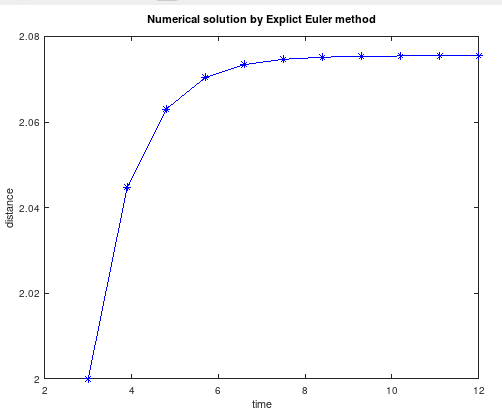
\includegraphics[width=9cm, height=4.5cm]{euler.png}
\end{figure}

\vspace{5mm}

\section{Implicit Euler Method}

\begin{minted}[frame=lines,framerule=3pt, framesep=10pt, fontsize=\small, linenos]{matlab}

% Initialization
f=@(t,y) exp(-t);

a=3;      b=12;
n=10;     h=(b-a)/n;    t=a:h:b;

y(1)=2;   % Inital guess

% Scheme
for i=1:n
  k(i)=f(t(i+1),y(i)+h*f(t(i),y(i)));
  y(i+1)=y(i)+h*k(i);

  fprintf('Solution at t=%d is %f.\n',t(i+1),y(i+1));
end

% Graph
plot(t,y,'-b*');
xlabel('time');   ylabel('distance');
title('Numerical solution by Implict Euler method');
\end{minted}
\clearpage

\section{Second order Runge-Kutta method}

\begin{minted}[frame=lines,framerule=3pt, framesep=10pt, fontsize=\small, linenos]{matlab}

% Initialization
f=@(t,y) exp(-t);

a=3;      b=12;
n=10;     h=(b-a)/n;    t=a:h:b;

y(1)=2;   % Inital guess

% Scheme
for i=1:n
  k(i)=f(t(i),y(i));
  k(i+1)=f(t(i+1),y(i)+h*k(i));

  y(i+1)=y(i)+0.5*h*(k(i)+k(i+1));

  fprintf('Solution at t=%d is %f.\n',t(i+1),y(i+1));
end

% Graph
plot(t,y,'-b*');
xlabel('time');   ylabel('distance');
title('Second order Runge-Kutta method');

\end{minted}
\clearpage

\section{Fourth order Runge-Kutta Method}

\begin{minted}[frame=lines,framerule=3pt, framesep=10pt, fontsize=\small, linenos]{matlab}

% Initialization
f=@(t,y) exp(-t);

a=3;      b=12;
n=10;     h=(b-a)/n;    t=a:h:b;

y(1)=2;   % Inital guess

% Scheme
for i=1:n
  k(i)=f(t(i),y(i));
  k(i+1)=f(t(i)+0.5*h,y(i)+0.5*h*k(i));
  k(i+2)=f(t(i)+0.5*h,y(i)+0.5*h*k(i+1));
  k(i+3)=f(t(i)+h,y(i)+h*k(i+2));

  y(i+1)=y(i)+(h/6)*(k(i)+2*k(i+1)+2*k(i+2)+k(i+3));

  fprintf('Solution at t=%d is %f.\n',t(i+1),y(i+1));
end

% Graph
plot(t,y,'-b*');
xlabel('time');   ylabel('distance');
title('Fourth order Runge-Kutta method');
\end{minted}


\chapter{Solution of System of Equations}
\section{Gauss Elimination Method}

\begin{minted}[frame=lines,framerule=3pt, framesep=10pt, fontsize=\small, linenos]{matlab}
% Initialization
A=[13,2,3; 2,15,1; 1,-1,10];    b=[46;33;25];
[n,n]=size(A);

% Non zero diagonal elements
for j=1:n-1                     %row1
  for i=j+1:n                   %row2
    if A(j,j)==0
      t=A(j,:);
      A(j,:)=A(i,:);
      A(i,:)=t;

      t=b(j,:);
      b(j,:)=b(i,:);
      b(i,:)=t;
    end
  end
end

%Forward elimination
for j=1:n-1                      %column jth
  for i=j+1:n                    %(j+1)th row
    m(i,j)=A(i,j)/A(j,j);
    A(i,:)=A(i,:)-m(i,j)*A(j,:);
    b(i,:)=b(i,:)-m(i,j)*b(j,:);
  end
end

%Backward substituion
x(n,:)=b(n,:)/A(n,n); %nth cordinate; i.e last row in 'x'

for i=n-1:-1:1
  x(i,:)=(b(i,:)-A(i,i+1:n)*x(i+1:n,:))/A(i,i);
end
x

\end{minted}
\(ans:\;\;x =2.7279,1.6766,2.3949\)\\
(same for Gauss-Jordan and Gauss-Seidel method aswell)

\section{Gauss Seidel Method}

\begin{minted}[frame=lines,framerule=3pt, framesep=10pt, fontsize=\small, linenos]{matlab}
% Initilaziion
A=[13,2,3; 2,15,1; 1,-1,10];    b=[46;33;25];
N=length(b);                    toll=0.0001;
x=zeros(N,1);                   y=zeros(N,1);

for j=1:100
  for i=1:N
    num=b(i)-A(i,1:i-1)*x(1:i-1)-A(i,i+1:N)*x(i+1:N);
    x(i)=num/A(i,i);
  end

  if abs(x-y)<toll
    fprintf('Iteration number is %d\n',j);
    break
  end
  y=x;
end
x

\end{minted}

\section{Gauss-Jordan Method}

\begin{minted}[frame=lines,framerule=3pt, framesep=10pt, fontsize=\small, linenos]{matlab}
% Initilaziion
A=[13,2,3,46; 2,15,1,33; 1,-1,10,25];
[m,n]=size(A);

% Non zero diagonal elements
for j=1:m-1                     %row1
  for i=j+1:m                   %row2
    if A(j,j)==0
      t=A(j,:);
      A(j,:)=A(i,:);
      A(i,:)=t;
    end
  end
end

%Forward elimination
for j=1:n-2      %column jth; n-2 cause last column is b.
  for i=j+1:m                   %(j+1)th row
    m(i,j)=A(i,j)/A(j,j);
    A(i,:)=A(i,:)-m(i,j)*A(j,:);
    b(i,:)=b(i,:)-m(i,j)*b(j,:);
  end
end
% Backward elimination
for j=n-1:-1:2     %n-1 is the last column excluding b.
  for i=j-1:-1:1
    A(i,:)=A(i,:)-A(j,:)*(A(i,j)/A(j,j));
  end
end

% making pivot element 1
for i=1:m
  A(i,:)=A(i,:)/A(i,i);
  x(i)=A(i,n);
end
x
\end{minted}

\chapter{Grading System}
\begin{minted}[frame=lines,framerule=3pt, framesep=10pt, fontsize=\small, linenos]{matlab}
% Internal Full Marks is 20 and final full marks is 30
I=input('Internal Marks Obtained:');
F=input('Final Marks Obtained:');

R=min(I,F/30*20*1.2);
fprintf('Revised Internal Marks is %2.2f.\n',R);

T=R+F;
fprintf('Total Marks Obtained is %2.2f.\n',T);

if I>20||F>30
  disp('Wrong Information.');
else
  if T>=45
    y='A';
  elseif T>=40
    y='A-';
  elseif T>=35
    y='B';
  elseif T>=30
    y='B-';
  else
    y='Fail';
  end
end
fprintf('The obtained grade is %s.\n',y)

\end{minted}




\end{document}


%%% Local Variables:
%%% mode: latex
%%% TeX-master: t
%%% End:
